%% 
%% Copyright 2007, 2008, 2009 Elsevier Ltd
%% 
%% This file is part of the 'Elsarticle Bundle'.
%% ---------------------------------------------
%% 
%% It may be distributed under the conditions of the LaTeX Project Public
%% License, either version 1.2 of this license or (at your option) any
%% later version.  The latest version of this license is in
%%    http://www.latex-project.org/lppl.txt
%% and version 1.2 or later is part of all distributions of LaTeX
%% version 1999/12/01 or later.
%% 
%% The list of all files belonging to the 'Elsarticle Bundle' is
%% given in the file `manifest.txt'.
%% 

%% Template article for Elsevier's document class `elsarticle'
%% with numbered style bibliographic references
%% SP 2008/03/01

\documentclass[preprint,12pt, a4paper]{elsarticle}



%% Use the option review to obtain double line spacing
%% \documentclass[authoryear,preprint,review,12pt]{elsarticle}

%% For including figures, graphicx.sty has been loaded in
%% elsarticle.cls. If you prefer to use the old commands
%% please give \usepackage{epsfig}

%% The amssymb package provides various useful mathematical symbols
%% \usepackage{amssymb}
\usepackage{hyperref}
\setlength{\parindent}{0pt}
%% The amsthm package provides extended theorem environments
%% \usepackage{amsthm}

%% The lineno packages adds line numbers. Start line numbering with
%% \begin{linenumbers}, end it with \end{linenumbers}. Or switch it on
%% for the whole article with \linenumbers.
% \usepackage{lineno}
\usepackage{tabularray}
\usepackage{float}
\usepackage[T1]{fontenc}
\usepackage{helvet}
\renewcommand{\familydefault}{\sfdefault}

\journal{SoftwareX}

\begin{document}


\renewcommand{\labelenumii}{\arabic{enumi}.\arabic{enumii}}

\begin{frontmatter}

 
%% Title, authors and addresses

%% use the tnoteref command within \title for footnotes;
%% use the tnotetext command for the associated footnote;
%% use the fnref command within \author or \address for footnotes;
%% use the fntext command for the associated footnote;
%% use the corref command within \author for corresponding author footnotes;
%% use the cortext command for the associated footnote;
%% use the ead command for the email address,
%% and the form \ead[url] for the home page:
%% \title{Title\tnoteref{label1}}
%% \tnotetext[label1]{}
%% \author{Name\corref{cor1}\fnref{label2}}
%% \ead{email address}
%% \ead[url]{home page}
%% \fntext[label2]{}
%% \cortext[cor1]{}
%% \address{Address\fnref{label3}}
%% \fntext[label3]{}

\title{quicR:\ An R Library for Streamlined Data Handling of Real-Time Quaking Induced Conversion Assays}

\author[label1,label2,label3]{Gage Rowden\corref{cor}}
\fntext[ ]{\textit{E-mail address: }rowde002@umn.edu}
\cortext[cor]{Corresponding author.}
\author[label1,label2,label3]{Peter Larsen}
\address[label1]{Department of Veterinary and Biomedical Sciences, University of Minnesota, USA.}
\address[label2]{Minnesota Center for Prion Research and Outreach, University of Minnesota, USA.}
\address[label3]{Priogen Corp., USA.}

\begin{abstract}
Real-time quaking induced conversion (RT-QuIC) has quickly become a valuable diagnostic tool for protein misfolding disorders such as Creutzfeldt-Jakob disease and Parkinson's disease. Given that the technology is relatively new, academic and industry standards for quality filtering data and high throughput analysis of results have yet to be fully established. The open source R library, quicR, was developed to provide a standardized approach to RT-QuIC data analysis.\ quicR provides functions, which can be easily integrated into existing R workflows, for data curation, analysis, and vizualization.
\end{abstract}

\begin{keyword}
%% keywords here, in the form: keyword \sep keyword
R package \sep{} RT-QuIC \sep{} prion \sep{} diagnostics \sep{} CJD \sep{} Parkinson's

%% PACS codes here, in the form: \PACS code \sep code

%% MSC codes here, in the form: \MSC code \sep code
%% or \MSC[2008] code \sep code (2000 is the default)

\end{keyword}

\end{frontmatter}

% \linenumbers

\section*{Metadata}

\begin{table}[ht]
    \fontsize{9}{9}\selectfont
    \begin{tabular}{|l|p{6.5cm}|p{6.5cm}|}
        \hline{}
        \textbf{Nr.} & \textbf{Code metadata description} & \textbf{Metadata} \\
        \hline{}
        C1 & Current code version & V2.1.0 \\
        \hline{}
        C2 & Permanent link to code/repository used for this code version & \url{https://github.com/gage1145/quicR} \\
        \hline{}
        C3  & Permanent link to Reproducible Capsule & \url{https://github.com/gage1145/quicR/releases/tag/v2.1.0}\\
        \hline{}
        C4 & Legal Code License & GPL-3 \\
        \hline{}
        C5 & Code versioning system used & git \\
        \hline{}
        C6 & Software code languages, tools, and services used & R \\
        \hline{}
        C7 & Compilation requirements, operating environments \& dependencies & R (>=4.1.0) \\
        \hline{}
        C8 & If available Link to developer documentation/manual & \url{https://cran.r-project.org/web/packages/quicR/quicR.pdf}\\
        \hline{}
        C9 & Support email for questions & rowde002@umn.edu\\
        \hline{}
    \end{tabular}
\caption{Code metadata}
\label{codeMetadata} 
\end{table}


\section{Motivation and significance}
    Real-time quaking induced conversion (RT-QuIC) is a cutting-edge diagnostic assay that has garnered significant attention for its ultra-sensitive detection of misfolded protein aggregates~\cite{Wilham2010, Atarashi2011}. The assay works by converting a recombinant protein substrate into an amyloid aggregate in the presence of a misfolded seed~\cite{Wilham2010, Orru2012, Orru2017, Orru2015, Bongianni2019, Dassanayake2016, Hwang2018, Groveman2018, Metrick2020}. The assay's sensitivity and specificity make RT-QuIC a promising tool for diagnosing diseases such as prion disorders and other protein misfolding pathologies~\cite{Fiorini2020, Franceschini2017, Picasso-Risso2022, Holz2021}. However, the relatively recent development and novelty of the assay have left a gap in widely accepted academic and industry standards for data analysis and interpretation~\cite{Rowden2023}.

    To address this gap, we introduce quicR, an open-source library, developed in R~\cite{R2024}, dedicated to the cleaning, analysis, and visualization of RT-QuIC data. By consolidating key metrics and providing robust analytical tools, quicR aims to standardize the analysis pipeline and foster reproducibility within the field of quaking induced assays including related assays such as Nano-QuIC~\cite{Christenson2023} and Micro-QuIC~\cite{Lee2024}. quicR is designed with both researchers and diagnosticians in mind, providing a user-friendly interface that integrates seamlessly with existing R workflows.

    While universal diagnostic criteria for RT-QuIC have yet to be established, certain analytical metrics have emerged as valuable tools for interpreting assay results and kinetics. These include:

    \begin{enumerate}
        \item Time-to-threshold (TtT): The time required for the fluorescence signal to exceed a predefined threshold \cite{Orru2015}.
        \item Rate of amyloid formation (RAF): A measure of the kinetics of aggregate growth, which provides insight into the relative quantity of misfolded seed \cite{Gallups2022}.
        \item Maxpoint ratio (MPR): A ratio-based metric measuring peak normalized fluorescence intensities \cite{Rowden2023}.
        \item Maximum slope (MS): The steepest rate of fluorescence increase, reflecting the most rapid phase of aggregation \cite{Henderson2015}.
    \end{enumerate}

    Together, these metrics enable researchers to characterize the kinetics of RT-QuIC reactions comprehensively, enhancing the rigor and reliability of diagnostic decisions.

    In addition to analytical tools, quicR provides flexible and customizable visualization capabilities. Leveraging the powerful ggplot2 library \cite{ggplot2016}, quicR enables users to generate high-quality, publication-ready figures. These visualizations can be further customized using the intuitive `+' syntax of ggplot2, allowing for tailored presentations of RT-QuIC data.

    By combining standardized metrics, advanced visualization tools, and a commitment to open source science, quicR serves as a foundational resource for the growing RT-QuIC community. Its goal is to empower researchers to analyze and present their data with clarity, consistency, and cohesion.

% \textit{In this section, we want you to introduce the scientific background and the motivation for developing the software.}
% 
% \begin{itemize}
%     \item \textit{Explain why the software is important and describe the exact (scientific) problem(s) it solves.}
%     \item \textit{Indicate in what way the software has contributed (or will contribute in the future) to the process of scientific discovery; if available, please cite a research paper using the software.}
%     \item \textit{Provide a description of the experimental setting. (How does the user use the software?)}
%     \item \textit{Introduce related work in literature (cite or list algorithms used, other software etc.).}
% \end{itemize}

\section{Software description}
    \subsection{Software architecture}
        quicR was developed to address the growing need for efficient data conversion, analysis, and visualization of RT-QuIC data (Figure \ref{fig:workflow}). With a focus on usability and reproducibility, the package is designed to standardize workflows and ensure compatibility across multiple laboratories. 
        % Its primary input format is data exported as Excel workbooks from the proprietary MARS software (BMG Labtech, Ortenberg, Germany), providing seamless integration with existing experimental workflows.
        \begin{figure}[ht]
            \caption{Workflow hierarchy of the quicR package. Blue nodes indicate steps where BMG software is needed. Purple nodes indicate functions dedicated to handling metadata. Red nodes are functions that acquire and manipulate raw data. Orange nodes are functions which calculate some metric. Finally, yellow nodes represent data analysis endpoints.}
            \centering
            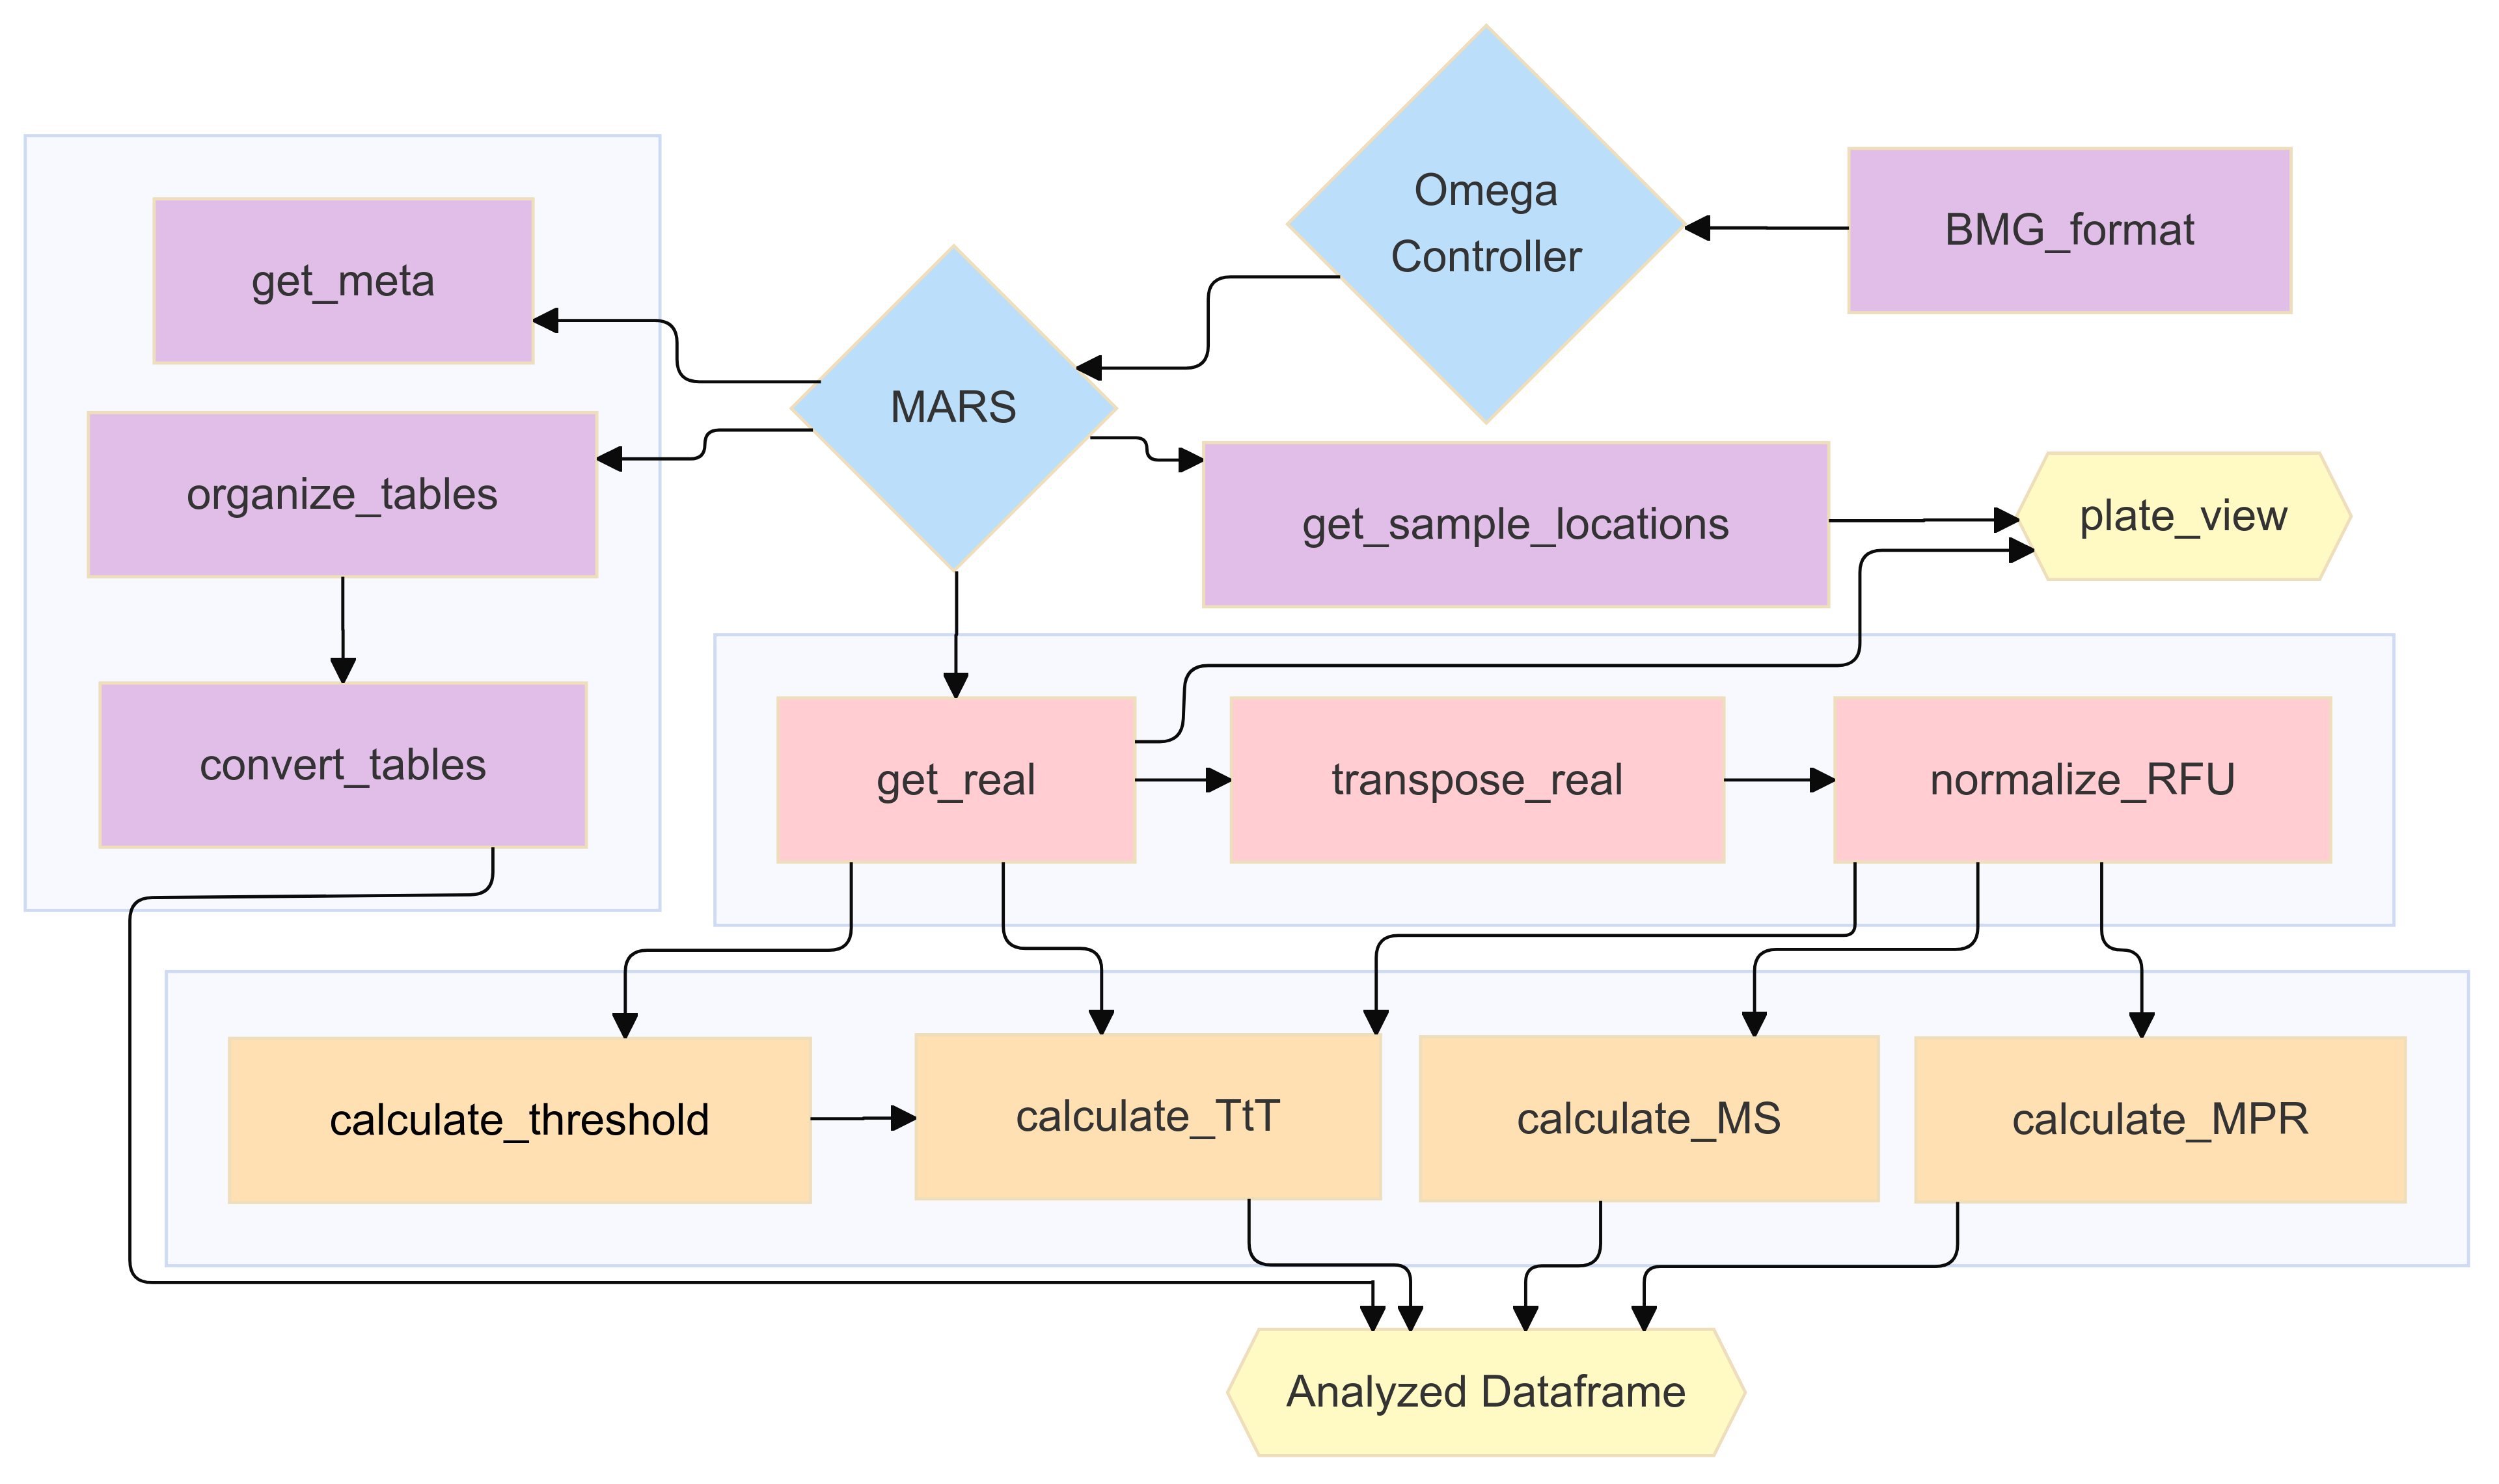
\includegraphics[width=\textwidth]{images/workflow2.png}
            \label{fig:workflow}
        \end{figure}

\subsection{Software functionalities}
    The implementation of the quicR package encompasses several streamlined processes designed to facilitate data input, cleaning, transformation, and analysis of RT-QuIC data. This section provides a comprehensive guide to utilizing the package's key functionalities, detailing how to:
        
    \begin{enumerate}
        \item Format and input sample data into Omega control software (BMG Labtech, Ortenberg, Germany).
        \item Extract, clean, and organize metadata and raw data and apply transformations and normalization for downstream analysis.
        \item Calculate critical analytical metrics, such as time-to-threshold (TtT), rate of amyloid formation (RAF), maxpoint ratio (MPR), and maximum slope (MS).
        \item Vizualize raw and analyzed data.
    \end{enumerate}

    These steps are designed to enhance reproducibility, minimize manual data handling, and enable seamless integration with the MARS software workflow. Through practical examples, this section illustrates how each function operates, along with expected input and output formats, ensuring clarity and ease of use for researchers.

    \subsubsection{Input of Sample IDs into Omega Control Software}
        \begin{enumerate}
            \item \textbf{BMG\_format()}: The Omega control software allows input of a TXT file containing sample IDs, dilution factors, and their well locations. This file is uniquely formatted, and not easily reproduced manually. This function allows for input of a CSV file containing the plate layout (see Table~\ref{tbl:layout} for proper formatting), and exports the formatted TXT file. The file can then be imported into the control software before running.
        \end{enumerate}
        
        \begin{table}[h]
            \caption{Example CSV file plate layout for input into the ``BMG\_format'' function. The top left corner should be cell ``A1'' in the CSV file. The top numbered row and the left-most lettered column should never be altered.\medskip}
            \label{tbl:layout}
            \begin{tblr}{
                colspec = {|c|cccccccccccc|}, 
                row{1} = {font=\bfseries}, 
                column{1} = {font=\bfseries}, 
                rowhead = 1
            }
                \hline
                & 1 & 2 & 3 & 4 & 5 & 6 & 7 & 8 & 9 & 10 & 11 & 12 \\ 
                \hline
                A & P & S01 & S02 & S03 & S04 & S05 & S06 & S07 & S08 & S09 & S10 & S11 \\ 
                B & P & S01 & S02 & S03 & S04 & S05 & S06 & S07 & S08 & S09 & S10 & S11 \\ 
                C & P & S01 & S02 & S03 & S04 & S05 & S06 & S07 & S08 & S09 & S10 & S11 \\ 
                D & P & S01 & S02 & S03 & S04 & S05 & S06 & S07 & S08 & S09 & S10 & S11 \\ 
                E & N & S01 & S02 & S03 & S04 & S05 & S06 & S07 & S08 & S09 & S10 & S11 \\ 
                F & N & S01 & S02 & S03 & S04 & S05 & S06 & S07 & S08 & S09 & S10 & S11 \\ 
                G & N & S01 & S02 & S03 & S04 & S05 & S06 & S07 & S08 & S09 & S10 & S11 \\ 
                H & N & S01 & S02 & S03 & S04 & S05 & S06 & S07 & S08 & S09 & S10 & S11 \\ 
                \hline
            \end{tblr}
        \end{table}

    % \subsection{Formatted Plate Layout for MARS input}
    %     The function, "BMG_format", includes the logical argument "write_file". If TRUE, it will create a TXT file. The path can be given to the "save_path" argument, and the file name can be supplied to the "save_name" argument. The text file will be formatted as follows, and can be imported into MARS.

    \subsubsection{Data Cleaning and Transformation}
        The MARS software (BMG Labtech, Ortenberg, Germany) exports real-time data as an Excel workbook. Typically, the first sheet in the workbook will include microplate views of both raw data and metadata; however, the metadata on this page is what is most useful for downstream processes. Those tables include the ``Sample IDa'' and ``Dilutions'' tables (if dilutions were included in the MARS export). For much of the downstream analysis, it is crucial that the ``Sample IDs'' table was exported from MARS.\@ If there is no table, the user can simply add it manually (see [@fig-sheet1] for proper formatting).

        \begin{enumerate}
            \item \textbf{organize\_tables()}: returns a list of tables contained in the first sheet of the exported Excel sheet. These tables contain valuable metadata such as sample IDs, dilution factors, and microplate locations.
            \item \textbf{convert\_tables()}: accepts the tables outputted from \textbf{organize\_tables} and converts them to columns in a dataframe.
            \item \textbf{get\_sample\_locations()}: extracts the well locations for each sample. Output of this function is used as an argument for vizualizing a microplate-level view of real-time data.
        \end{enumerate}
            % The metadata is defined as either sample-dependent or -independent. Sample-dependent metadata includes information such as sample IDs and dilution factors, whereas sample-independent metadata includes the date, time, reaction ID, etc.

            % The dependent metadata can be retrieved using the ``organize\_tables'' and ``convert\_tables'' functions. The former returns a list of tables, and the latter converts each table into a column in a single data frame.

        % \subsubsection{Sample Locations}
        %     Samples locations can be extracted based on their well ID.\@ The ``get\_sample\_locations'' function accepts additional arguments if dilution factors were exported from MARS.\@ The ``dilution\_bool'' argument can be set to TRUE if dilutions are to be included in the output. The ``dilution\_fun'' argument will supply a function for transforming the dilution factors (e.g.\ if the user would want to perform a log transformation). The user can supply a delimiter using the ``sep'' argument. The output of this function is critical as an argument in the ``plate\_view'' function which is further explained in the visualization section.

            % \subsubsection{Sample-Independent Metadata}
    \subsection{Retrieving and Manipulating Raw Data}
        The raw, real-time data is typically found on the second sheet of the Excel workbook exported from MARS. There are three functions dedicated to the retrieval and cleaning of raw data.

    \begin{enumerate}
        \item \textbf{get\_real()}: Retrieves the raw data from the Excel file, and outputs it as a dataframe.
        \item \textbf{transpose\_real()}: Swaps the rows and columns which makes some downstream analyses easier.
        \item \textbf{normalize\_RFU()}: normalizes the raw data by dividing each read by background fluorescence at a given cycle.
    \end{enumerate}

        % \subsubsection{Retrieve Raw Data}
        %     Raw data can be retrieved using the ``get\_real'' function. The logical argument, ``ordered'', indicates whether the user would prefer the columns to be ordered by well or by sample ID.\@ By default, it is FALSE which will order the data by well. This should almost always be the case for easier integration with other downstream functions. Additionally, since there can be more than one instance of real-time data (depending on if the user added some calculations in MARS), ``get\_real'' returns a list of dataframes. Therefore, the output must be indexed to access the data frame of interest.

        % \subsubsection{Transpose Raw Data}
        %     This data is structured such that each sample is its own column (variable) and each row (observation) is a time point. While this format is technically correct, a transposed format is more ideal for some downstream manipulation. This operation is performed using the function, ``transpose\_real''. After transposition, each time point is an individual column (variable), and each sample is an individual row (observation).

        % \subsubsection{Normalize Raw Data}
        %     The function ``normalize\_RFU'' will convert the raw data into a background normalized data set. The function includes two additional arguments, ``bg\_cycle'' (the cycle which will be used as the background fluorescence value) and ``transposed'' (if FALSE, will make a call to the ``transpose\_real'' function). Note that the fourth time point is all ``1's'' since this was designated the background cycle.

    \subsection{Calculations}
        There are three analytical metrics with dedicated functions: time-to-threshold (TtT), maxpoint ratio (MPR), and maximum slope (MS). The rate of amyloid formation does not have a designated function since it is simply the reciprocal of the time-to-threshold (1/TtT). Each function below accepts input from the ``transpose\_real'' or the ``normalize\_RFU'' functions. See Figure \ref{fig:metrics} for an example of the output of these functions.

        \begin{enumerate}
            \item \textbf{calculate\_threhold()}: returns a value which is a given number of standard deviations above the average background fluorescence of the entire microplate.
            % Many publications have different methods of determining thresholds. By convention, the most popular method is to take the average background fluorescence of the every well and add some multiple of standard deviations~\cite{Rowden2023}. The quicR package provides the ``calculate\_threshold'' function for this purpose. A value can be provided as the optional argument, ``multiplier'', which will be applied to the standard deviation.

            \item \textbf{calculate\_TtT()}: takes the real-time data and calculates the time in hours needed to reach a given threshold value.
            % TtT is calculated using the ``calculate\_TtT'' function. The function must be supplied a threshold; default value is 2 (i.e.\ twice the background fluorescence if the data is normalized). A starting column should also be given as an integer; default value is 3. This is essentially asking how many columns of metadata are included before the fluorescence reads begin. 

            % TtT is calculated by iterating through each row and checking if a value is greater than the threshold. If the value is greater, the slope of the previous time-point to the current time-point is calculated, and the time intersection of the current read is returned.

            \item \textbf{calculate\_MPR()}: accepts raw or normalized data and returns the maximum value obtained during the run. If supplied with raw data, it will make a call to the normalize\_RFU() function.
            % MPR is calculated by the ``calculate\_MPR'' function. Data must be normalized in order to derive this metric. In a normalized data set, the MPR is simply the maximum value achieved during the run. Raw data can be passed to this function, but the argument ``data\_is\_norm'', must be set to FALSE.\ This will pass the raw data to ``normalize\_RFU'' before calculating the MPR values.

            \item \textbf{calculate\_MS()}: computes the approximate derivative of the real-time data and returns the maximum value obtained during the run.
            % MS is calculated by the ``calculate\_MS'' function. The function iterates through each row using a rolling window which can be adjusted (default value is 3). Given the window size, the slope is calculated based on change in fluorescence divided by the range of the window. The MS is simply the largest slope value recorded. The units are typically reported as $\Delta$RFU/h.
        \end{enumerate}

        \begin{figure}[h]
            \caption{}
            \centering{}
            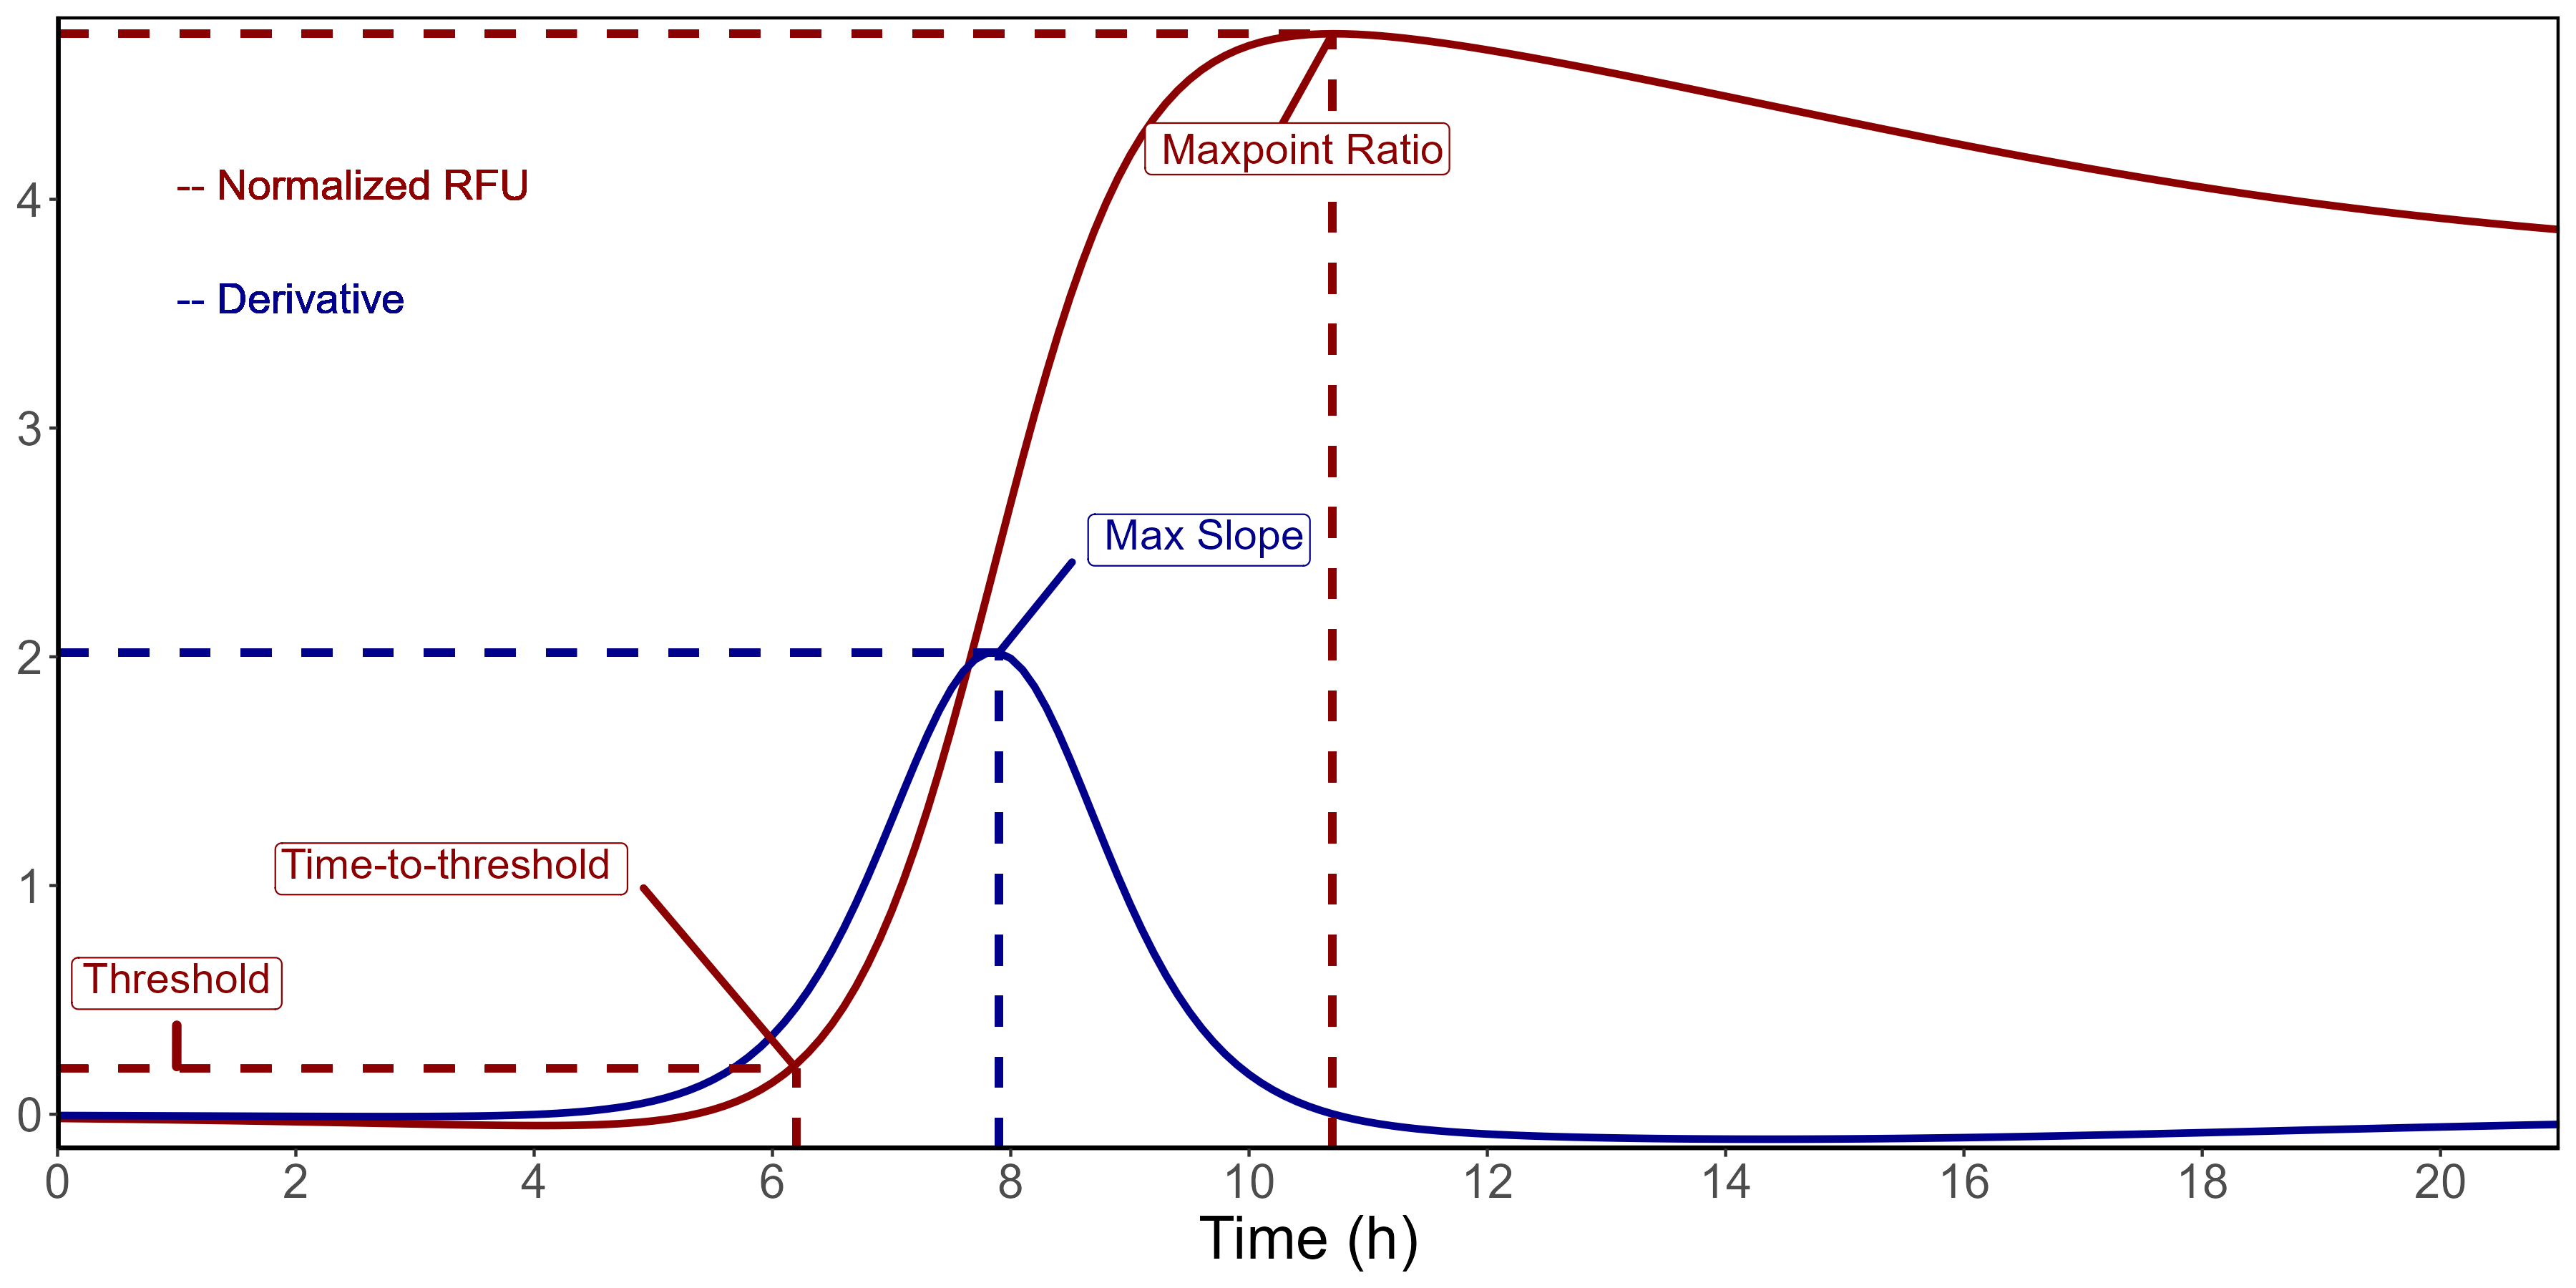
\includegraphics[width=\textwidth]{images/metric_example.png}
            \label{fig:metrics}
        \end{figure}

    \subsection{Vizualization}
        
    
    % \subsection{Sample code snippets analysis (optional)}
\section{Illustrative examples}

% \textit{Provide at least one illustrative example to demonstrate the major
% functions of your software/code.}

% \textit{\textbf{Optional}: you may include one explanatory  video or screencast that will appear next to your article, in the right hand side panel. Please upload any video as a single supplementary file with your article. Only one MP4 formatted, with 150MB maximum size, video is possible per article. Recommended video dimensions are 640 x 480 at a maximum of 30 frames / second. Prior to submission please test and validate your .mp4 file at  \url{http://elsevier-apps.sciverse.com/GadgetVideoPodcastPlayerWeb/verification} . This tool will display your video exactly in the same way as it will appear on ScienceDirect. }

\section{Impact}
% \textit{This is the main section of the article and reviewers will weight it appropriately.
% Please indicate:}
% \begin{itemize}
%     \item \textit{Any new research questions that can be pursued as a result of your software.}
%     \item \textit{In what way, and to what extent, your software improves the pursuit of existing research questions.}
%     \item \textit{Any ways in which your software has changed the daily practice of its users.}
%     \item \textit{How widespread the use of the software is within and outside the intended user group (downloads, number of users if your software is a service, citable publications, etc.).}
%     \item \textit{How the software is being used in commercial settings and/or how it has led to the creation of spin-off companies.}
%     \end{itemize}
% \textit{Please note that points 1 and 2 are best demonstrated by
%   references to citable publications.}

\section{Conclusions}
    quicR offers a powerful solution for the cleaning, analysis, and visualization of RT-QuIC data, addressing critical needs in a rapidly evolving field. By enabling consistent data handling and interpretation, quicR lays the groundwork for improved diagnostic consistency and reproducibility. The package's open-source nature ensures that it will continue to evolve, integrating new insights and technologies as they emerge.

    As RT-QuIC technology advances, tools like quicR will play a pivotal role in bridging the gap between assay development and practical application. By equipping researchers with reliable, standardized tools, quicR not only supports the study of prion and protein misfolding disorders but also serves as a model for the development of software solutions in other diagnostic fields.

\section*{Acknowledgements}
\label{}
Special thanks to Beni Altmann at The Comprehensive R Archive Network (CRAN) for help during the submission process to CRAN. We thank Tiffany Wolf and Marc Schwabenlander for their support through the Minnesota Center for Prion Research and Outreach. We would like to acknowledge Suzanne Stone and Sarah Gresch for maintaining lab operations.


%% The Appendices part is started with the command \appendix;
%% appendix sections are then done as normal sections
%% \appendix

%% \section{}
%% \label{}

%% References:
%% If you have bibdatabase file and want bibtex to generate the
%% bibitems, please use
%%
\bibliographystyle{elsarticle-num} 
\bibliography{references.bib}

% \textit{If the software repository you used supplied a DOI or another
% Persistent IDentifier (PID), please add a reference for your software
% here. For more guidance on software citation, please see our guide for
% authors or \href{https://f1000research.com/articles/9-1257/v2}{this
%   article on the essentials of software citation by FORCE 11}, of
% which Elsevier is a member.}

% \large{\textbf{Reminder: Before you submit, please delete all 
% the instructions in this document, 
% including this paragraph. 
% Thank you!}}





\end{document}
\endinput
%%
%% End of file `SoftwareX_article_template.tex'.

%%% Local Variables:
%%% mode: latex
%%% TeX-master: t
%%% End:
